% Options for packages loaded elsewhere
\PassOptionsToPackage{unicode}{hyperref}
\PassOptionsToPackage{hyphens}{url}
%
\documentclass[
  10pt,
]{report}
\usepackage{amsmath,amssymb}
\usepackage{lmodern}
\usepackage{iftex}
\ifPDFTeX
  \usepackage[T1]{fontenc}
  \usepackage[utf8]{inputenc}
  \usepackage{textcomp} % provide euro and other symbols
\else % if luatex or xetex
  \usepackage{unicode-math}
  \defaultfontfeatures{Scale=MatchLowercase}
  \defaultfontfeatures[\rmfamily]{Ligatures=TeX,Scale=1}
  \setmainfont[]{Times New Roman}
\fi
% Use upquote if available, for straight quotes in verbatim environments
\IfFileExists{upquote.sty}{\usepackage{upquote}}{}
\IfFileExists{microtype.sty}{% use microtype if available
  \usepackage[]{microtype}
  \UseMicrotypeSet[protrusion]{basicmath} % disable protrusion for tt fonts
}{}
\makeatletter
\@ifundefined{KOMAClassName}{% if non-KOMA class
  \IfFileExists{parskip.sty}{%
    \usepackage{parskip}
  }{% else
    \setlength{\parindent}{0pt}
    \setlength{\parskip}{6pt plus 2pt minus 1pt}}
}{% if KOMA class
  \KOMAoptions{parskip=half}}
\makeatother
\usepackage{xcolor}
\IfFileExists{xurl.sty}{\usepackage{xurl}}{} % add URL line breaks if available
\IfFileExists{bookmark.sty}{\usepackage{bookmark}}{\usepackage{hyperref}}
\hypersetup{
  hidelinks,
  pdfcreator={LaTeX via pandoc}}
\urlstyle{same} % disable monospaced font for URLs
\usepackage[left = 1in, right = 1in, top = 1in, bottom = 1in]{geometry}
\usepackage{longtable,booktabs,array}
\usepackage{calc} % for calculating minipage widths
% Correct order of tables after \paragraph or \subparagraph
\usepackage{etoolbox}
\makeatletter
\patchcmd\longtable{\par}{\if@noskipsec\mbox{}\fi\par}{}{}
\makeatother
% Allow footnotes in longtable head/foot
\IfFileExists{footnotehyper.sty}{\usepackage{footnotehyper}}{\usepackage{footnote}}
\makesavenoteenv{longtable}
\usepackage{graphicx}
\makeatletter
\def\maxwidth{\ifdim\Gin@nat@width>\linewidth\linewidth\else\Gin@nat@width\fi}
\def\maxheight{\ifdim\Gin@nat@height>\textheight\textheight\else\Gin@nat@height\fi}
\makeatother
% Scale images if necessary, so that they will not overflow the page
% margins by default, and it is still possible to overwrite the defaults
% using explicit options in \includegraphics[width, height, ...]{}
\setkeys{Gin}{width=\maxwidth,height=\maxheight,keepaspectratio}
% Set default figure placement to htbp
\makeatletter
\def\fps@figure{htbp}
\makeatother
\setlength{\emergencystretch}{3em} % prevent overfull lines
\providecommand{\tightlist}{%
  \setlength{\itemsep}{0pt}\setlength{\parskip}{0pt}}
\setcounter{secnumdepth}{5}
\newlength{\cslhangindent}
\setlength{\cslhangindent}{1.5em}
\newlength{\csllabelwidth}
\setlength{\csllabelwidth}{3em}
\newlength{\cslentryspacingunit} % times entry-spacing
\setlength{\cslentryspacingunit}{\parskip}
\newenvironment{CSLReferences}[2] % #1 hanging-ident, #2 entry spacing
 {% don't indent paragraphs
  \setlength{\parindent}{0pt}
  % turn on hanging indent if param 1 is 1
  \ifodd #1
  \let\oldpar\par
  \def\par{\hangindent=\cslhangindent\oldpar}
  \fi
  % set entry spacing
  \setlength{\parskip}{#2\cslentryspacingunit}
 }%
 {}
\usepackage{calc}
\newcommand{\CSLBlock}[1]{#1\hfill\break}
\newcommand{\CSLLeftMargin}[1]{\parbox[t]{\csllabelwidth}{#1}}
\newcommand{\CSLRightInline}[1]{\parbox[t]{\linewidth - \csllabelwidth}{#1}\break}
\newcommand{\CSLIndent}[1]{\hspace{\cslhangindent}#1}
%General Formatting
\usepackage{setspace}\doublespacing %Double Spacing
\usepackage{sectsty}\allsectionsfont{\normalsize} % Make all font size 12
\usepackage[all]{nowidow} %Prevent "orphans and widows"
\usepackage{booktabs} %Publication quality tables

%Table of Contents, List of Tables, List of Figures
\usepackage[titles]{tocloft} %Load package for customizing table of contents/lists/figures (Adding titles makes it so that they are formatted the same as chapter titles)
\renewcommand{\contentsname}{Table of Contents} %Rename Contents to Table of Contents
\renewcommand{\cftchapleader}{\cftdotfill{\cftdotsep}} % dots for chapters in table of contents
\renewcommand{\cfttoctitlefont}{\normalsize\bfseries} %Bold faced normal size font for title of Table of Contents
\renewcommand{\cftloftitlefont}{\normalsize\bfseries} %Bold faced normal size font for title of List of Tables
\renewcommand{\cftlottitlefont}{\normalsize\bfseries} %Bold faced normal size font for List of Tables
\renewcommand{\cftchapfont}{\normalsize} %Unbold chapter titles in table of contents
\renewcommand{\cftchappagefont}{\normalfont} %Unbold chapter page numbers in table of contents
%\renewcommand{\cftchappresnum}{Chapter~} %Precede number with "Chapter"
%\renewcommand{\cftchapnumwidth}{2cm} %Add space between Chapter number and title
\renewcommand{\cftfigpresnum}{Figure~} %Precede number with "Figure"
\renewcommand{\cftfignumwidth}{2.5cm} %Add space between figure number and caption must offset for hanging caption below
\renewcommand{\cftfigaftersnumb}{\hspace{-0.635cm}} %handing 0.25 in indent for long caption second line
\renewcommand{\cfttabpresnum}{Table~}  %Precede number with "Table"
\renewcommand{\cfttabnumwidth}{2.5cm} %Add space between table number and caption need to offset for hang indent below
\renewcommand{\cfttabaftersnumb}{\hspace{-0.635cm}} %hanging indent for table captions that take up more than one line
\renewcommand{\cftchapindent}{0in} %Set indents to increase by 0.5 inches per level (level 1)
\renewcommand{\cftsecindent}{0.5in} %Set indents to increase by 0.5 inches per level (level 2)
\renewcommand{\cftsecnumwidth}{1.5cm} %off set hanging indent for long section lines below (level 2)
\renewcommand{\cftsecaftersnumb}{\hspace{-0.635cm}} %hanging indent for sections that take up more than one line (level 2)
\renewcommand{\cftsubsecindent}{1in} %Set indents to increase by 0.5 inches per level (level 3)
\renewcommand{\cftsubsecnumwidth}{1.5cm} %off set hanging indent for long section lines below (level 3)
\renewcommand{\cftsubsecaftersnumb}{\hspace{-0.635cm}}%hanging indent for sections that take up more than one line (level 3)
\renewcommand{\cftsubsubsecindent}{1.5in} %Set indents to increase by 0.5 inches per level (level 4)
\renewcommand{\cftsubsubsecnumwidth}{1.8cm} %off set hanging indent for long section lines below (level 4)
\renewcommand{\cftsubsubsecaftersnumb}{\hspace{-0.635cm}}%hanging indent for sections that take up more than one line (level 4)
\renewcommand{\cftparaindent}{2in} %Set indents to increase by 0.5 inches per level (level 5)
\renewcommand{\cftparanumwidth}{2.1cm} %off set hanging indent for long section lines below (level 5)
\renewcommand{\cftparaaftersnumb}{\hspace{-0.635cm}}%hanging indent for sections that take up more than one line (level 5)
\renewcommand{\cftsubparaindent}{2.5in} %Set indents to increase by 0.5 inches per level (level 6)
\renewcommand{\cftsubparanumwidth}{2.4cm} %off set hanging indent for long section lines below (level 6)
\renewcommand{\cftsubparaaftersnumb}{\hspace{-0.635cm}}%hanging indent for sections that take up more than one line (level 6)



\makeatletter
\renewcommand\@tocrmarg{0.5in} % Make long titles wrap when they are 0.5 inches away from page numbers
\makeatother

\newcommand*{\noaddvspace}{\renewcommand*{\addvspace}[1]{}}
\addtocontents{lof}{\protect\noaddvspace} %Prevents gap between chapters in List of Figures
\addtocontents{lot}{\protect\noaddvspace} %Prevents gap between chapters in List of Tables

%Chapter Headings
\usepackage{titlesec}
\titleformat{\chapter}[hang] %Make chapter number and title on same line
{\normalfont\normalsize\bfseries}{\chaptertitlename\ \thechapter:}{1em}{} %Adjust title font formatting (normal, bold)
\titlespacing{\chapter}{0pt}{40pt}{12pt} %{increases the left margin}{vertical space before the title}{separation between title and text}
\titlespacing{\part}{0pt}{35pt}{12pt} %{increases the left margin}{vertical space before the title}{separation between title and text}

%Appendix
%\usepackage[titletoc]{appendix}

\usepackage{tocloft}
\usepackage{calc}
\renewcommand{\cftchappresnum}{\chaptername\space}
%\setlength{\cftchapnumwidth}{\widthof{\textbf{Appendix~999~}}}
\setlength{\cftchapnumwidth}{2.635cm}
\renewcommand{\cftchapaftersnumb}{\hspace{-0.635cm}}
\makeatletter
\g@addto@macro\appendix{%
  \addtocontents{toc}{%
    \protect\renewcommand{\protect\cftchappresnum}{\appendixname\space}%
  }%
}
\newcommand*\annex{%
  \renewcommand{\appendixname}{Annex}%
  \setcounter{chapter}{0}
  \addtocontents{toc}{%
    \protect\renewcommand{\protect\cftchappresnum}{\appendixname\space}%
  }%
}

\usepackage{blindtext}% only for dummy text
%https://tex.stackexchange.com/questions/435684/how-to-include-appendix-names-in-toc
\usepackage{booktabs}
\usepackage{longtable}
\usepackage{array}
\usepackage{multirow}
\usepackage{wrapfig}
\usepackage{float}
\usepackage{colortbl}
\usepackage{pdflscape}
\usepackage{tabu}
\usepackage{threeparttable}
\usepackage{threeparttablex}
\usepackage[normalem]{ulem}
\usepackage{makecell}
\usepackage{xcolor}
\ifLuaTeX
  \usepackage{selnolig}  % disable illegal ligatures
\fi

\author{}
\date{\vspace{-2.5em}}

\begin{document}

\hypertarget{dedication}{%
\chapter*{Dedication}\label{dedication}}

Placeholder

\hypertarget{abstract}{%
\chapter*{Abstract}\label{abstract}}
\addcontentsline{toc}{chapter}{Abstract}

This is a quick summary of what I found. This is a quick summary of what I found. This is a quick summary of what I found. This is a quick summary of what I found. This is a quick summary of what I found. This is a quick summary of what I found. This is a quick summary of what I found. This is a quick summary of what I found. This is a quick summary of what I found. This is a quick summary of what I found.

\pagenumbering{arabic}

\hypertarget{introduction}{%
\section{Introduction}\label{introduction}}

General background information and your literature review goes here. General background information and your literature review goes here. General background information and your literature review goes here. General background information and your literature review goes here. General background information and your literature review goes here. General background information and your literature review goes here. General background information and your literature review goes here. General background information and your literature review goes here. General background information and your literature review goes here. General background information and your literature review goes here. General background information and your literature review goes here.

\hypertarget{methods}{%
\section{Methods}\label{methods}}

This is how I did the thing with this data (Table \ref{tab:testtable})

\begin{table}

\caption{\label{tab:testtable}Summary of the mtcars data.}
\centering
\begin{tabular}[t]{lll}
\toprule
  &     speed &      dist\\
\midrule
 & Min.   : 4.0 & Min.   :  2.00\\
 & 1st Qu.:12.0 & 1st Qu.: 26.00\\
 & Median :15.0 & Median : 36.00\\
 & Mean   :15.4 & Mean   : 42.98\\
 & 3rd Qu.:19.0 & 3rd Qu.: 56.00\\
\addlinespace
 & Max.   :25.0 & Max.   :120.00\\
\bottomrule
\end{tabular}
\end{table}

\hypertarget{results}{%
\section{Results}\label{results}}

\hypertarget{level-3}{%
\subsection{Level 3}\label{level-3}}

\hypertarget{level-4}{%
\subsubsection{Level 4}\label{level-4}}

\hypertarget{level-5}{%
\paragraph{Level 5}\label{level-5}}

\hypertarget{level-6-super-long-header-to-make-sure-it-works-at-different-levels-just-in-case}{%
\subparagraph{Level 6 Super long header to make sure it works at different levels just in case}\label{level-6-super-long-header-to-make-sure-it-works-at-different-levels-just-in-case}}

\hypertarget{a-really-long-heading-so-i-see-what-happens-when-it-takes-up-more-than-one-line-just-in-case-were-getting-crazy}{%
\subsection{A Really Long Heading so I see what happens when it takes up more than one line just in case we're getting crazy}\label{a-really-long-heading-so-i-see-what-happens-when-it-takes-up-more-than-one-line-just-in-case-were-getting-crazy}}

These are my first results (Figure \ref{fig:cars-plot}).

\begin{figure}
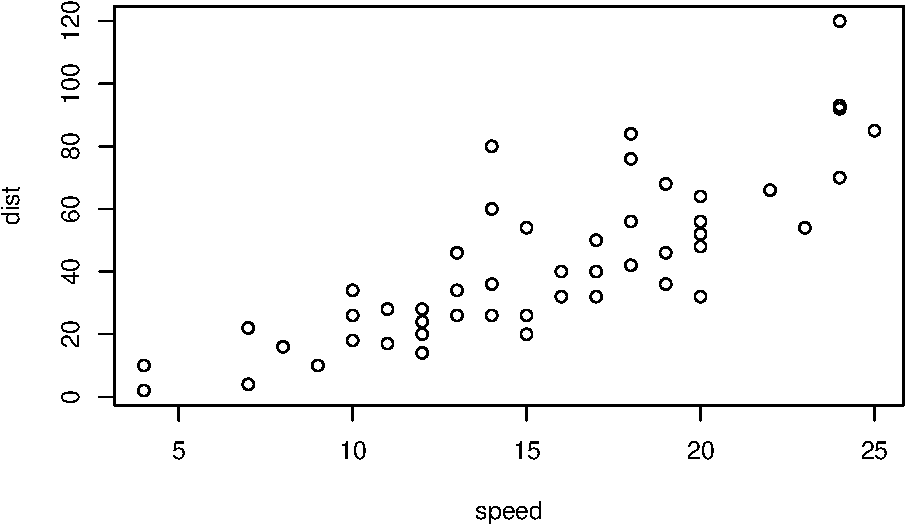
\includegraphics{Dissertation_files/figure-latex/cars-plot-1} \caption[The cars data.]{The cars data. Sentence two.}\label{fig:cars-plot}
\end{figure}

And then I also got these results (Figure \ref{fig:test-fig}).

\begin{figure}
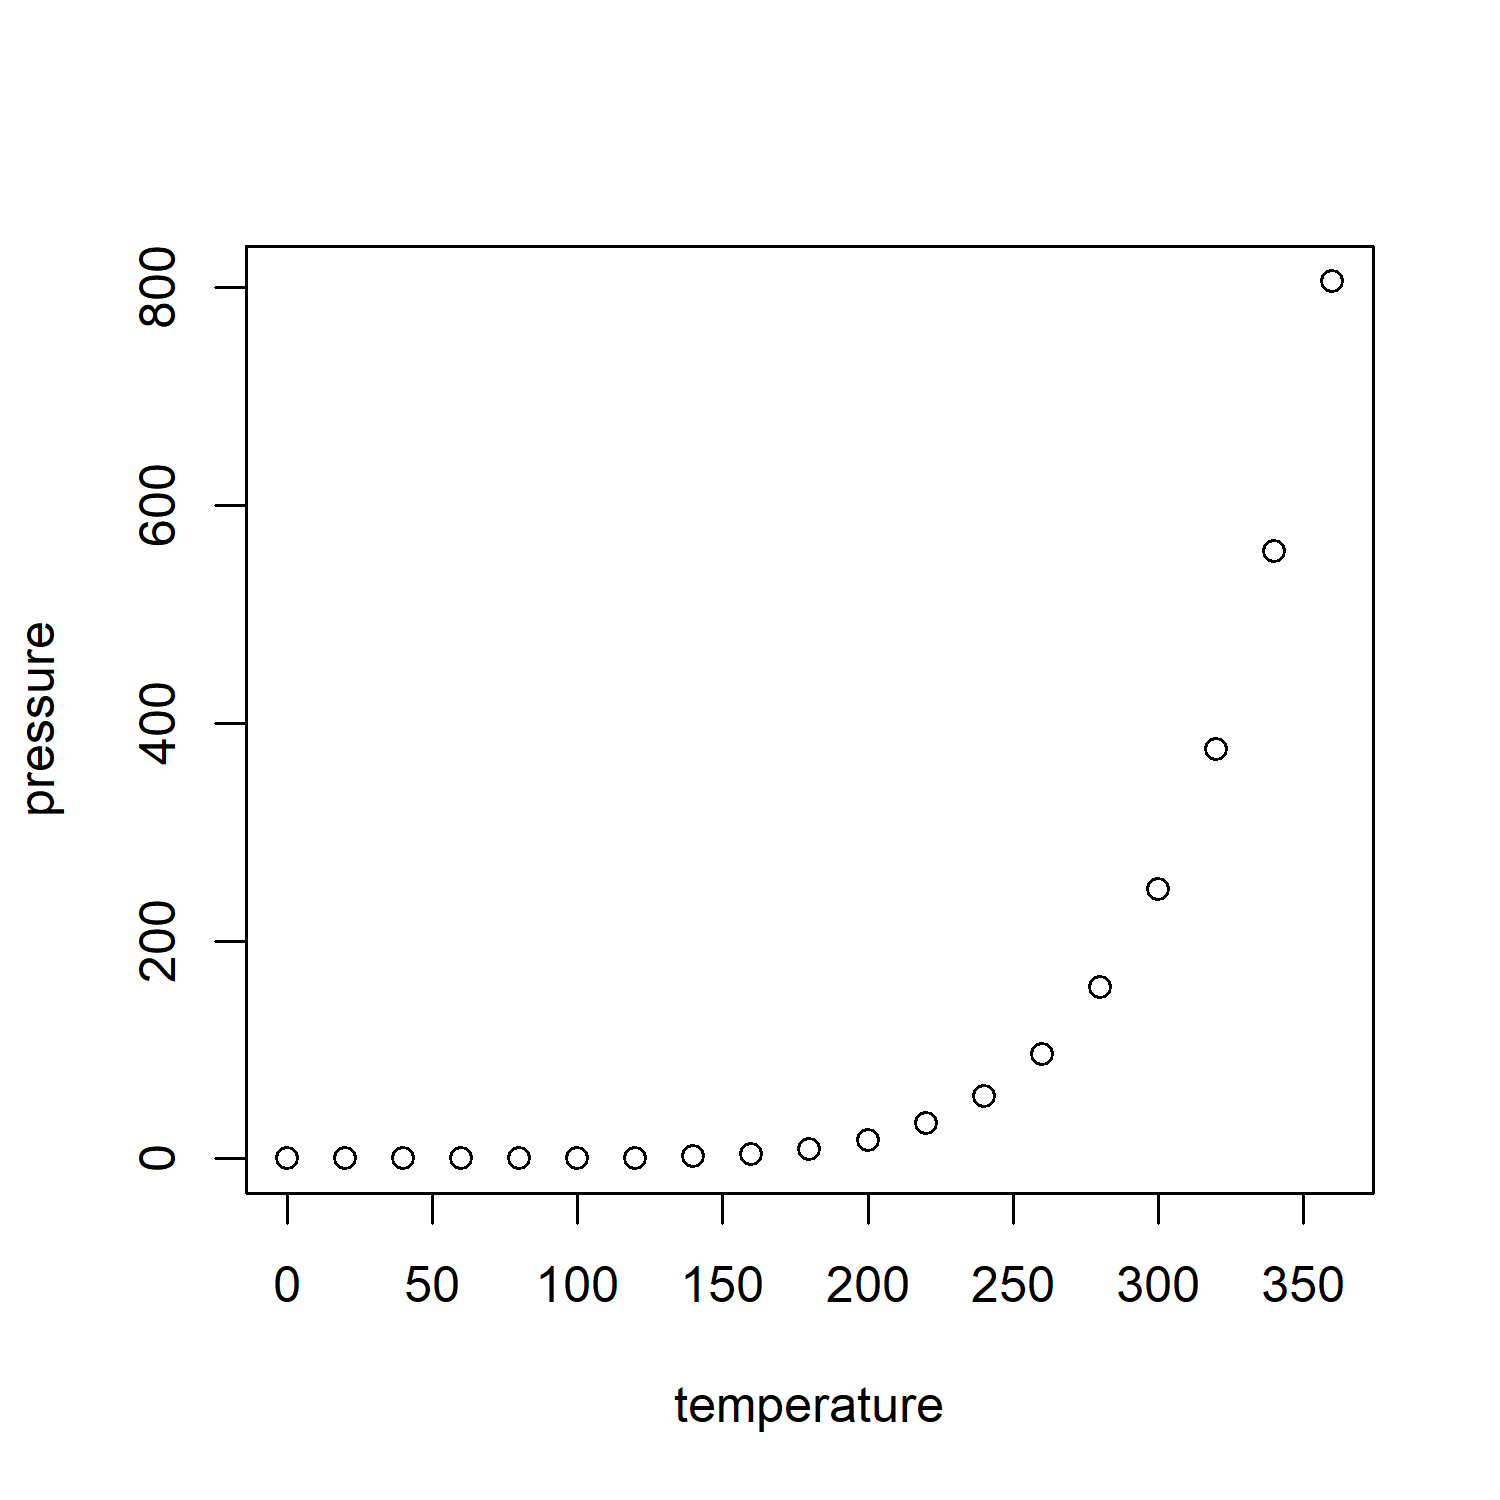
\includegraphics[width=20.83in]{Figures/pressure_plot} \caption{A really long figure caption so I see what happens when it takes up more than one line just in case we're getting crazy}\label{fig:test-fig}
\end{figure}

\begin{table}

\caption{\label{tab:testtable-2}A really long table caption so I see what happens when it takes up more than one line just in case we're getting crazy}
\centering
\begin{tabular}[t]{r|r}
\hline
speed & dist\\
\hline
4 & 2\\
\hline
4 & 10\\
\hline
7 & 4\\
\hline
7 & 22\\
\hline
8 & 16\\
\hline
9 & 10\\
\hline
\end{tabular}
\end{table}

\hypertarget{discussion}{%
\section{Discussion}\label{discussion}}

Now I tell you how this fits in the context of my field

\hypertarget{my-chapter-title}{%
\chapter{My Chapter Title}\label{my-chapter-title}}

Placeholder

\hypertarget{introduction-1}{%
\section{Introduction}\label{introduction-1}}

\hypertarget{methods-1}{%
\section{Methods}\label{methods-1}}

\hypertarget{results-1}{%
\section{Results}\label{results-1}}

\hypertarget{an-equation-and-some-math}{%
\subsection{An Equation and some math}\label{an-equation-and-some-math}}

\hypertarget{discussion-1}{%
\section{Discussion}\label{discussion-1}}

\hypertarget{my-chapter-title-1}{%
\chapter{My Chapter Title}\label{my-chapter-title-1}}

\hypertarget{synthesis}{%
\section{Synthesis}\label{synthesis}}

Everything fits together so well!

\hypertarget{future-work}{%
\section{Future Work}\label{future-work}}

Ok it didn't fit together so well so I guess we should look at these things, but I have to graduate and there's no more money but maybe someone some day can look into this.

\hypertarget{references}{%
\chapter*{References}\label{references}}
\addcontentsline{toc}{chapter}{References}

\hypertarget{refs}{}
\begin{CSLReferences}{0}{0}
\end{CSLReferences}

\hypertarget{appendix-appendix}{%
\appendix}


\hypertarget{name-of-appendix}{%
\chapter{Name of Appendix}\label{name-of-appendix}}

\begin{figure}
\centering
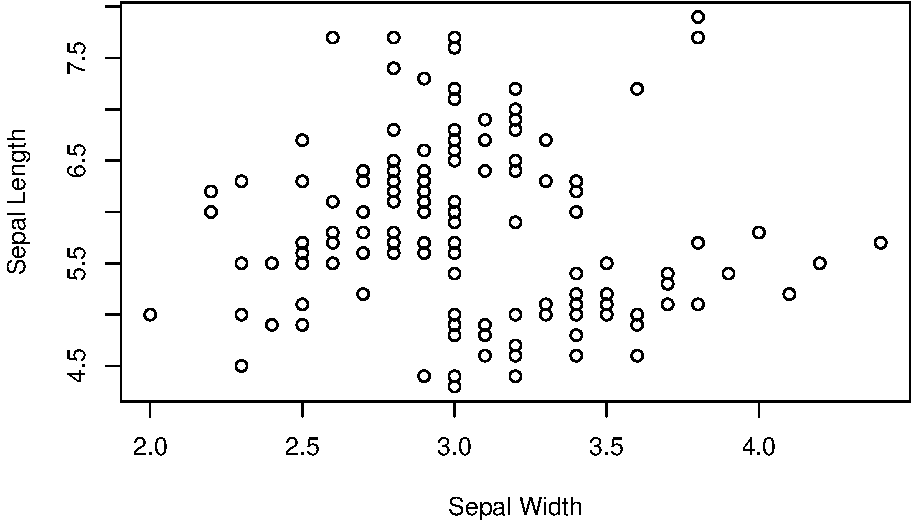
\includegraphics{Dissertation_files/figure-latex/iris-data-fig-1.pdf}
\caption{\label{fig:iris-data-fig}sepal length vs sepal width of the iris data.}
\end{figure}

\hypertarget{name-of-appendix-1}{%
\chapter{Name of Appendix}\label{name-of-appendix-1}}

\begin{table}[!h]

\caption{\label{tab:iris-data}The iris data}
\centering
\fontsize{8}{10}\selectfont
\begin{tabular}[t]{r|r|r|r|l}
\hline
Sepal.Length & Sepal.Width & Petal.Length & Petal.Width & Species\\
\hline
5.1 & 3.5 & 1.4 & 0.2 & setosa\\
\hline
4.9 & 3.0 & 1.4 & 0.2 & setosa\\
\hline
4.7 & 3.2 & 1.3 & 0.2 & setosa\\
\hline
4.6 & 3.1 & 1.5 & 0.2 & setosa\\
\hline
5.0 & 3.6 & 1.4 & 0.2 & setosa\\
\hline
5.4 & 3.9 & 1.7 & 0.4 & setosa\\
\hline
4.6 & 3.4 & 1.4 & 0.3 & setosa\\
\hline
5.0 & 3.4 & 1.5 & 0.2 & setosa\\
\hline
4.4 & 2.9 & 1.4 & 0.2 & setosa\\
\hline
4.9 & 3.1 & 1.5 & 0.1 & setosa\\
\hline
5.4 & 3.7 & 1.5 & 0.2 & setosa\\
\hline
4.8 & 3.4 & 1.6 & 0.2 & setosa\\
\hline
4.8 & 3.0 & 1.4 & 0.1 & setosa\\
\hline
4.3 & 3.0 & 1.1 & 0.1 & setosa\\
\hline
5.8 & 4.0 & 1.2 & 0.2 & setosa\\
\hline
5.7 & 4.4 & 1.5 & 0.4 & setosa\\
\hline
5.4 & 3.9 & 1.3 & 0.4 & setosa\\
\hline
5.1 & 3.5 & 1.4 & 0.3 & setosa\\
\hline
5.7 & 3.8 & 1.7 & 0.3 & setosa\\
\hline
5.1 & 3.8 & 1.5 & 0.3 & setosa\\
\hline
5.4 & 3.4 & 1.7 & 0.2 & setosa\\
\hline
5.1 & 3.7 & 1.5 & 0.4 & setosa\\
\hline
4.6 & 3.6 & 1.0 & 0.2 & setosa\\
\hline
5.1 & 3.3 & 1.7 & 0.5 & setosa\\
\hline
4.8 & 3.4 & 1.9 & 0.2 & setosa\\
\hline
\end{tabular}
\end{table}

\end{document}
